\chapter{Chapter 6. Conclusions and Future Work}

\section{Combined results}
Figures \ref{fig:histogram-duration} and \ref{fig:histogram-scalesize} show the distributions of event duration and structure scale size from events identified with wavelet analysis and the GS-based method. The scale sizes of the solar wind events and the magnetosheath events have a large difference, in part because of the differences in duration. The wavelet events in the solar wind are almost twice as large as the events from the GS-based method. In the magnetosheath, the average scale size of the wavelet events is almost three times as large as that of the GS events. Because of the difference in the minimum and maximum limits of calculating the duration of the events between the wavelet analysis and GS-based methods, the ranges in duration are different. The range of duration for the SFRs identified by the wavelet analysis method is dictated by the time cadence of the spacecraft data \citep{Torrence:1998}; whereas the duration range of the SFRs identified by the GS-based method can be extended arbitrarily toward the upper limit end (though there are computational limits). The scale size is calculated by taking the average speed of the event interval and multiplying it by the duration of the event for the wavelet analysis. For the SFRs identified by the GS-based method, this calculation is done using the projected de Hoffmann-Teller frame velocity on the cross-sectional plane, which takes into account the orientation of the cylindrical structure in relation to the spacecraft path thus representing a better cross-sectional size. Whereas such a characterization is not feasible through the wavelet analysis method because like a typical time-series analysis method, it does not characterize structure in dimensions higher than 1D. The scale size calculated in the GS-based method represents a true cross-sectional size for a 2D configuration. 

Figure \ref{fig:histogram-scalesize} shows the corresponding distributions of the scale sizes for the identified events in the magnetosheath and solar wind. They generally follow power laws and the trends indicate that there are more, smaller-size events in the magnetosheath than in the solar wind. This is largely seen through the slope of the scale size distribution of the GS-based method in the magnetosheath, which has a smaller upper limit and a steeper slope than the corresponding distribution in the solar wind. The power-law distributions in Figure \ref{fig:histogram-scalesize} can indicate anomalous (super- or sub- diffusive) transport. Solar energetic particles (SEPs) can be trapped between the boundaries of two adjacent SFRs \citep{leRoux:2023}, but with power law distributions of SFR scale sizes, the energetic particles can escape to open field lines, i.e., super-diffusive transport. The power law distributions in this work support the theory that when there is energetic particle transport through coherent magnetic structures that create strong, intermittent magnetic fields, the distributions yield a non-Gaussian power law \citep{leRoux:2021}.

\begin{figure}
    \centering
    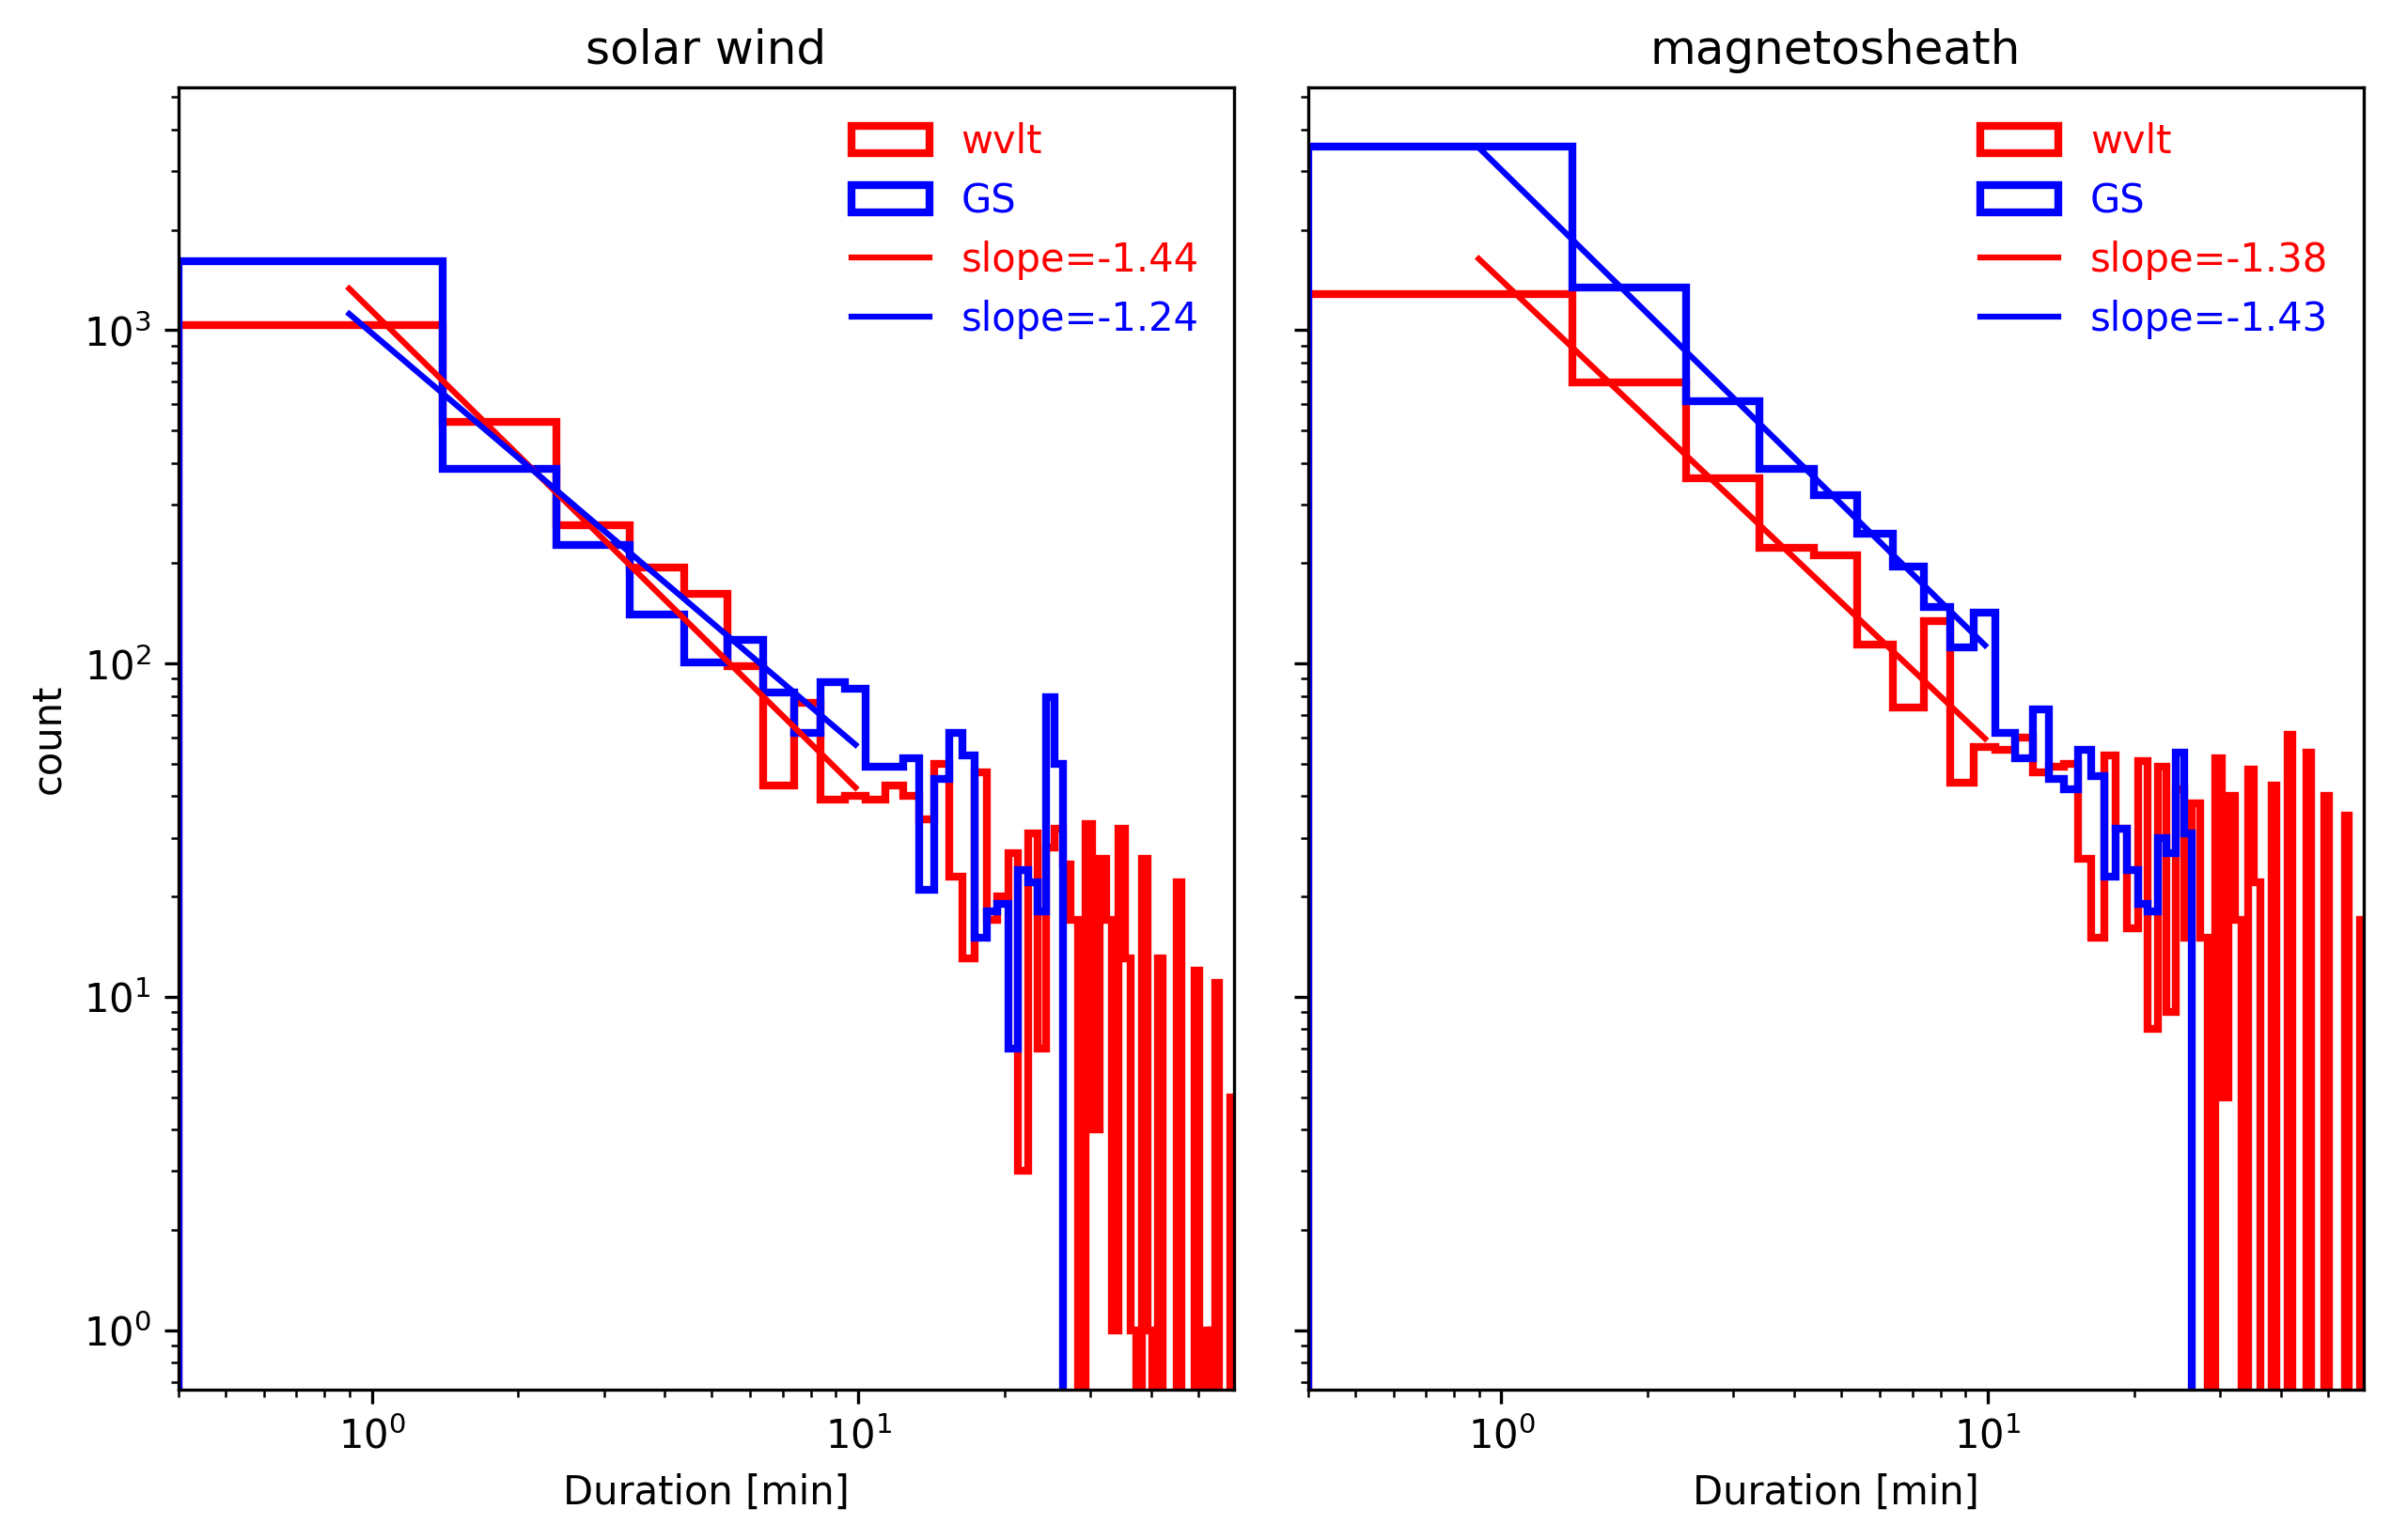
\includegraphics[width=\textwidth]{Figures/Histograms/histogram_duration.png}
    \caption[Histograms of duration for identified events]{Histograms of the duration of events identified by using wavelet analysis (red lines) and the GS-based method (blue lines) in the solar wind (left panel) and magnetosheath (right panel), respectively. The straight lines are the nominal linear fitting to each distribution in a log-log scale with the corresponding slopes denoted in the legend.}
    \label{fig:histogram-duration}
\end{figure}

\begin{figure}
    \centering
    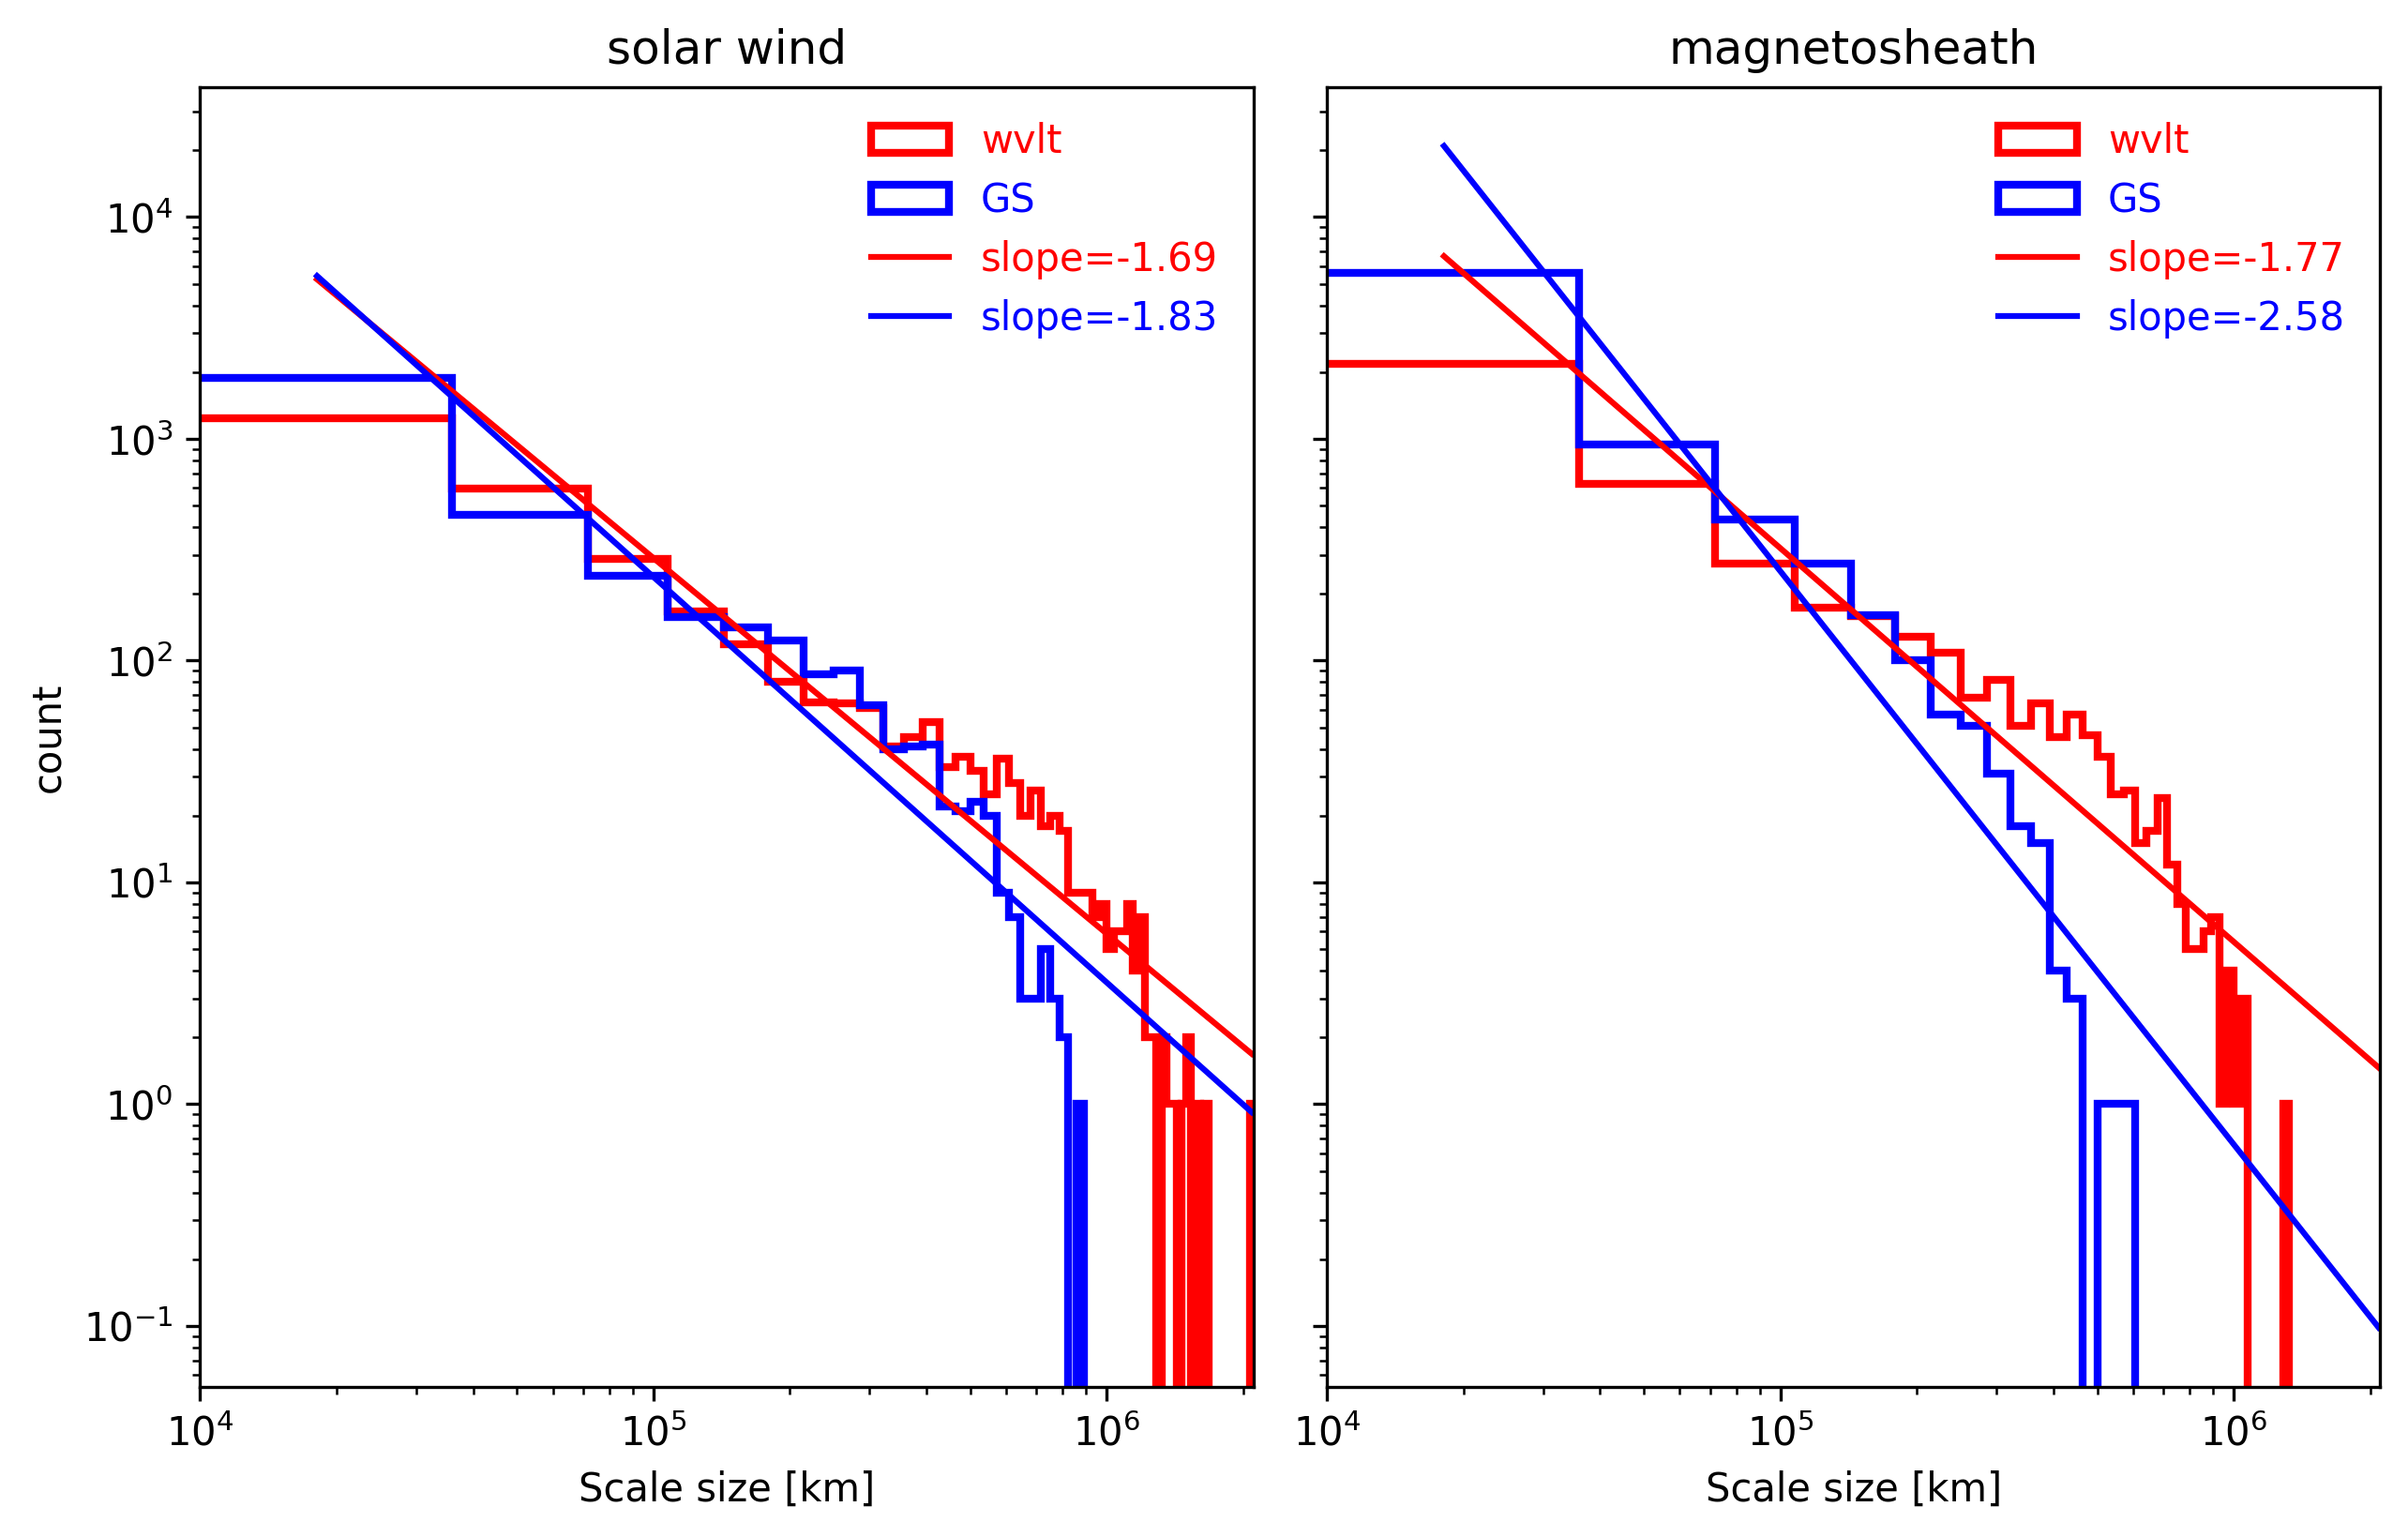
\includegraphics[width=\textwidth]{Figures/Histograms/histogram_scalesize.png}
    \caption[Histograms of scale size for identified events]{Same as Figure \ref{fig:histogram-duration} but for scale size distributions of identified events.}
    \label{fig:histogram-scalesize}
\end{figure}

\begin{figure}
    \centering
    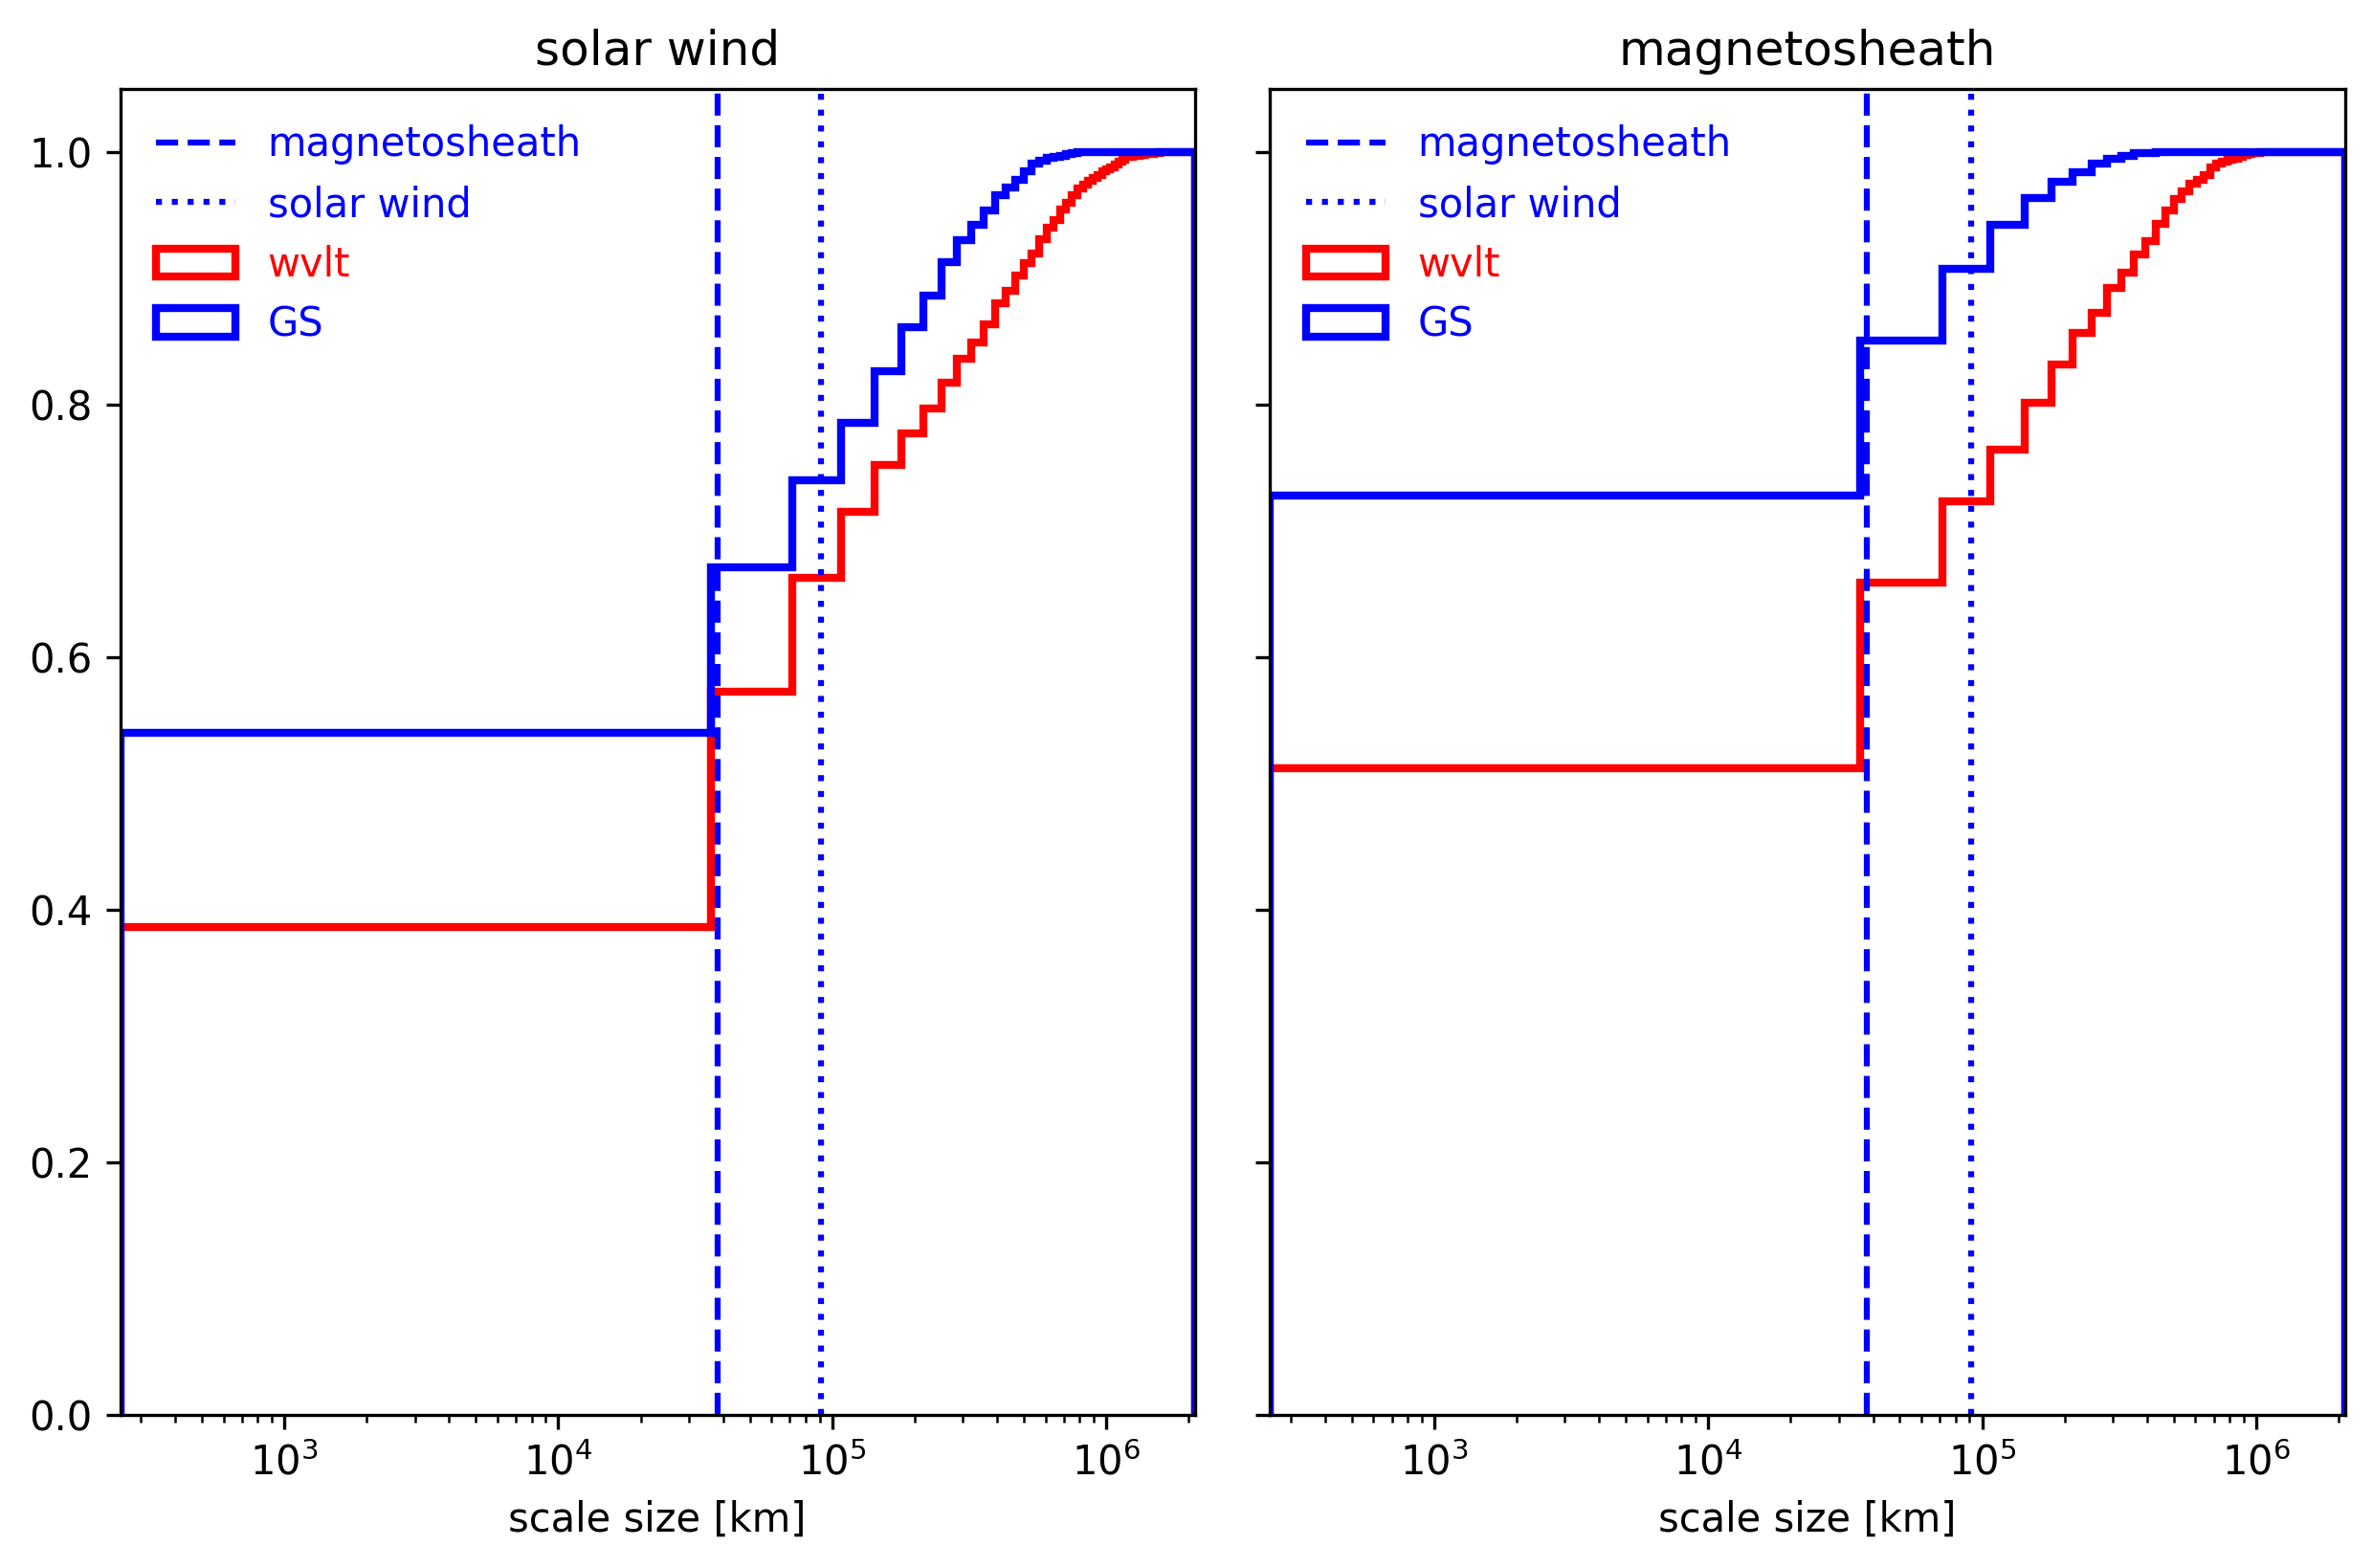
\includegraphics[width=\textwidth]{Figures/Histograms/cdf_scalesize.png}
    \caption[Cumulative distribution function of scale sizes for the identified events]{Cumulative distribution function of scale sizes for the identified events (see legend) in the solar wind (left panel) and magnetosheath (right panel). The vertical lines mark the corresponding mean values of the scale sizes for the GS-based method for the solar wind (dotted blue lines) and the magnetosheath (dashed blue lines) in both panels.}
    \label{fig:cdf-scalesize}
\end{figure}

In Figure \ref{fig:cdf-scalesize}, the cumulative distribution functions of the scale sizes further show that there is a larger percentage of smaller structures in the magnetosheath than in the solar wind. For instance in the magnetosheath, the percentage of events with scale sizes smaller than the mean value (marked by the dashed line in both panels) is greater than 70\% which is significantly larger than the corresponding percentage in the solar wind. The structures generally seem to be compressed across the bow shock: the scale sizes are smaller, and the magnetic field becomes stronger. Furthermore, the maximum scale size of the SFRs in the solar wind is found to be approximately 2 million km, which is on the same order as the turbulence correlation length \citep{Horbury:1996}. The power-law distributions are also in agreement with \citep{Nakanotani:2022, Nakanotani2:2022} which simulated the generation and interaction of smaller scale structures across a shock wave and compared with the turbulence theory \citep{Zank:2021, Zank:2017}. Based on our analysis result, since the solar wind is dominated by quasi-2D structures, such as SFRs, the power laws are generally in agreement with the 2D-slab model of turbulence \citep{Zank:2021, Zank:2017}.


\begin{figure}
    \centering
    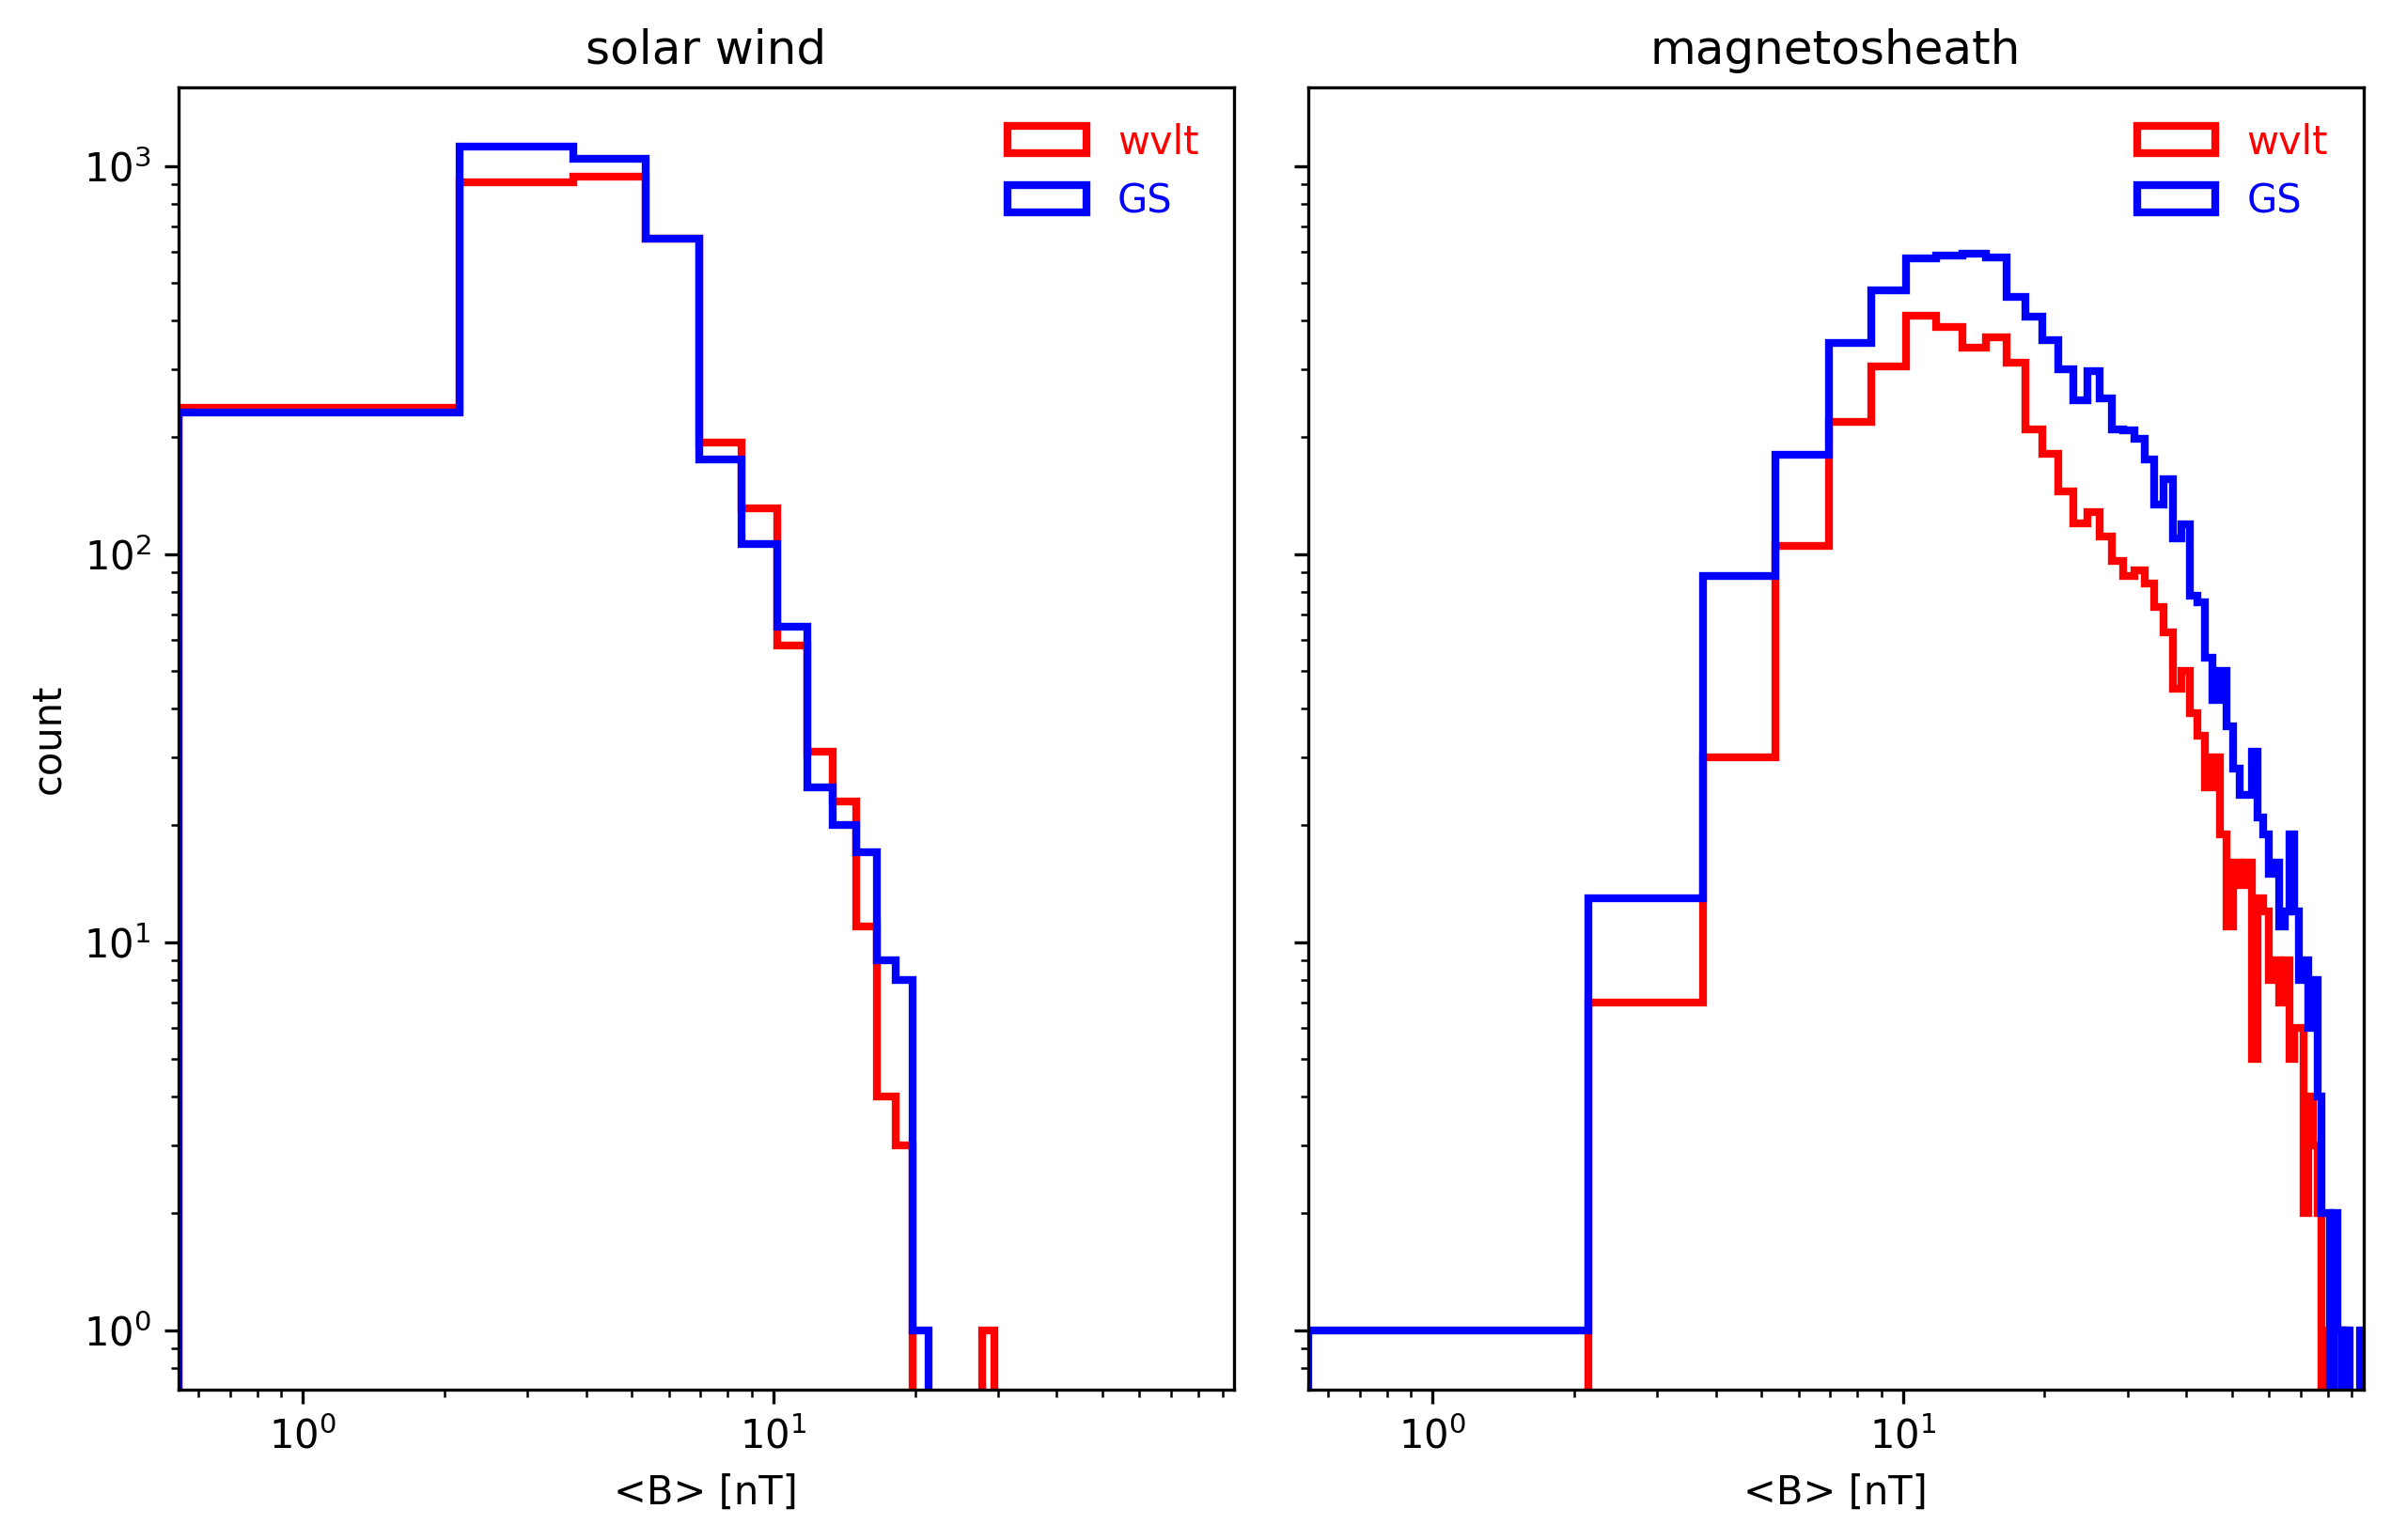
\includegraphics[width=\textwidth]{Figures/Histograms/histogram_Bfield.png}
    \caption[Histograms of average magnetic field for identified events]{Same as Figure \ref{fig:histogram-duration} but for average magnetic field distributions of identified events.}
    \label{fig:histogram-Bfield}
\end{figure}

\begin{figure}
    \centering
    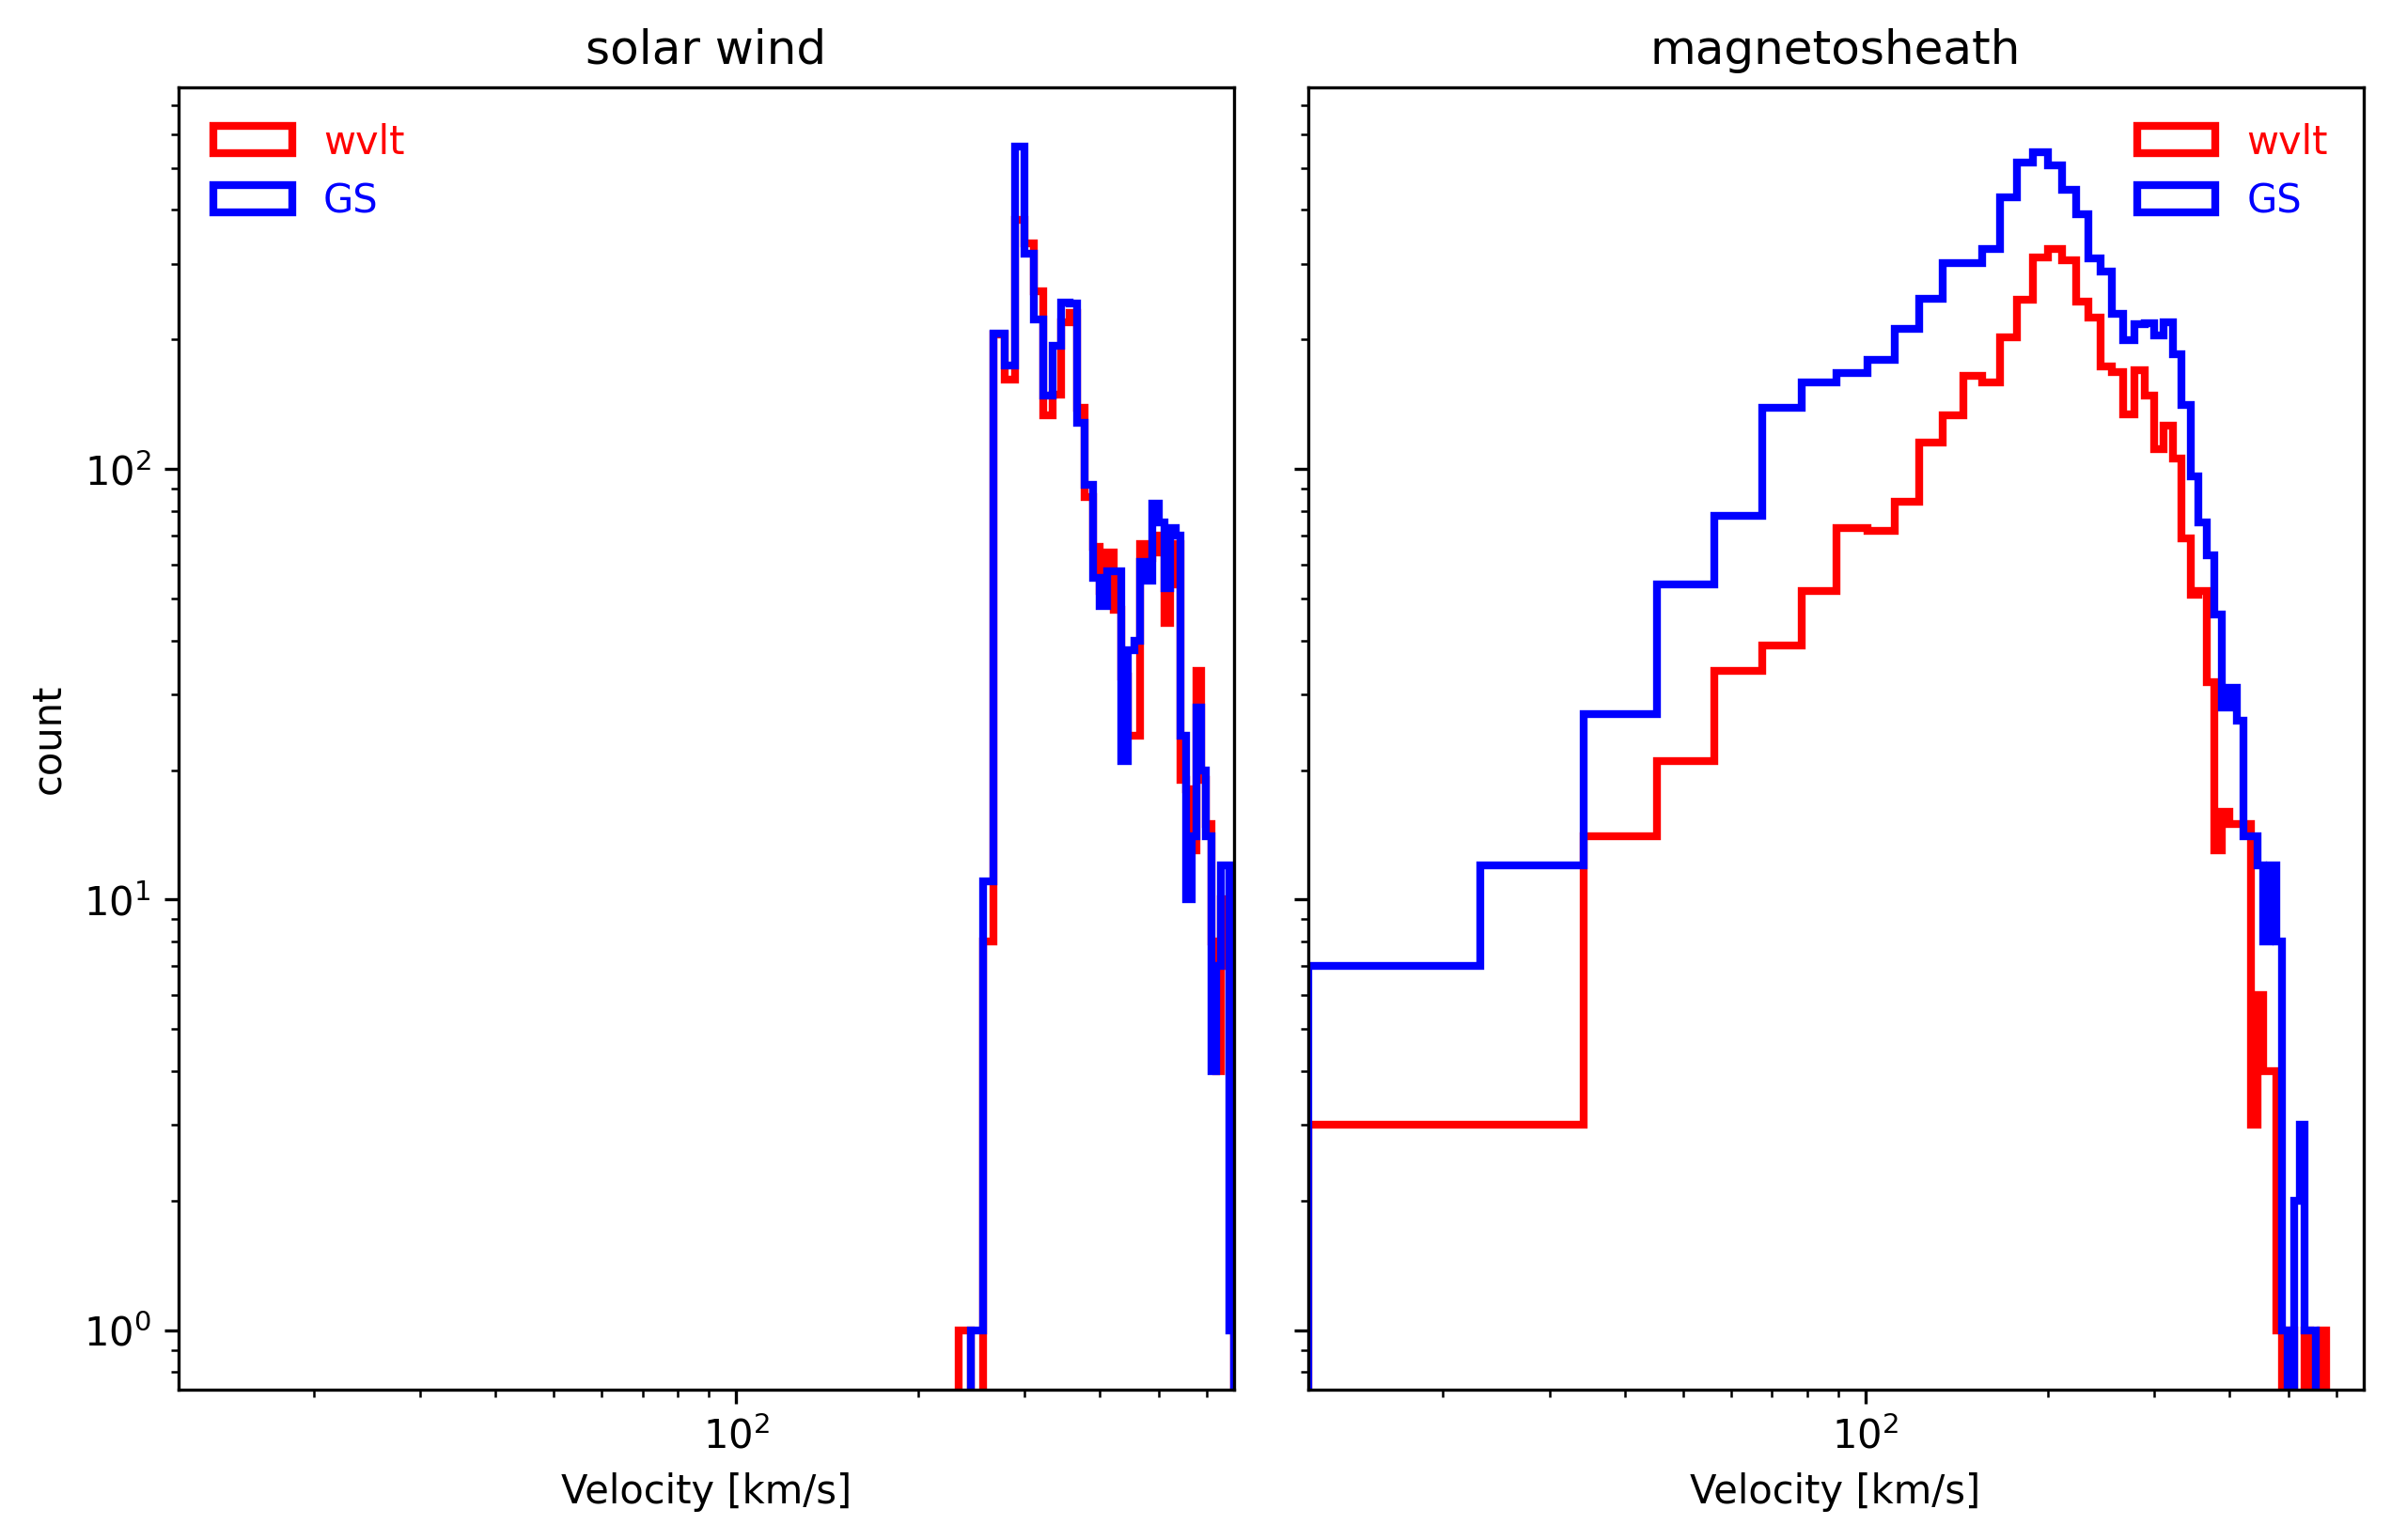
\includegraphics[width=\textwidth]{Figures/Histograms/histogram_velocity.png}
    \caption[Histograms of velocity for identified events]{Same as Figure \ref{fig:histogram-duration} but for velocity distributions of identified events.}
    \label{fig:histogram-velocity}
\end{figure}

\begin{figure}
    \centering
    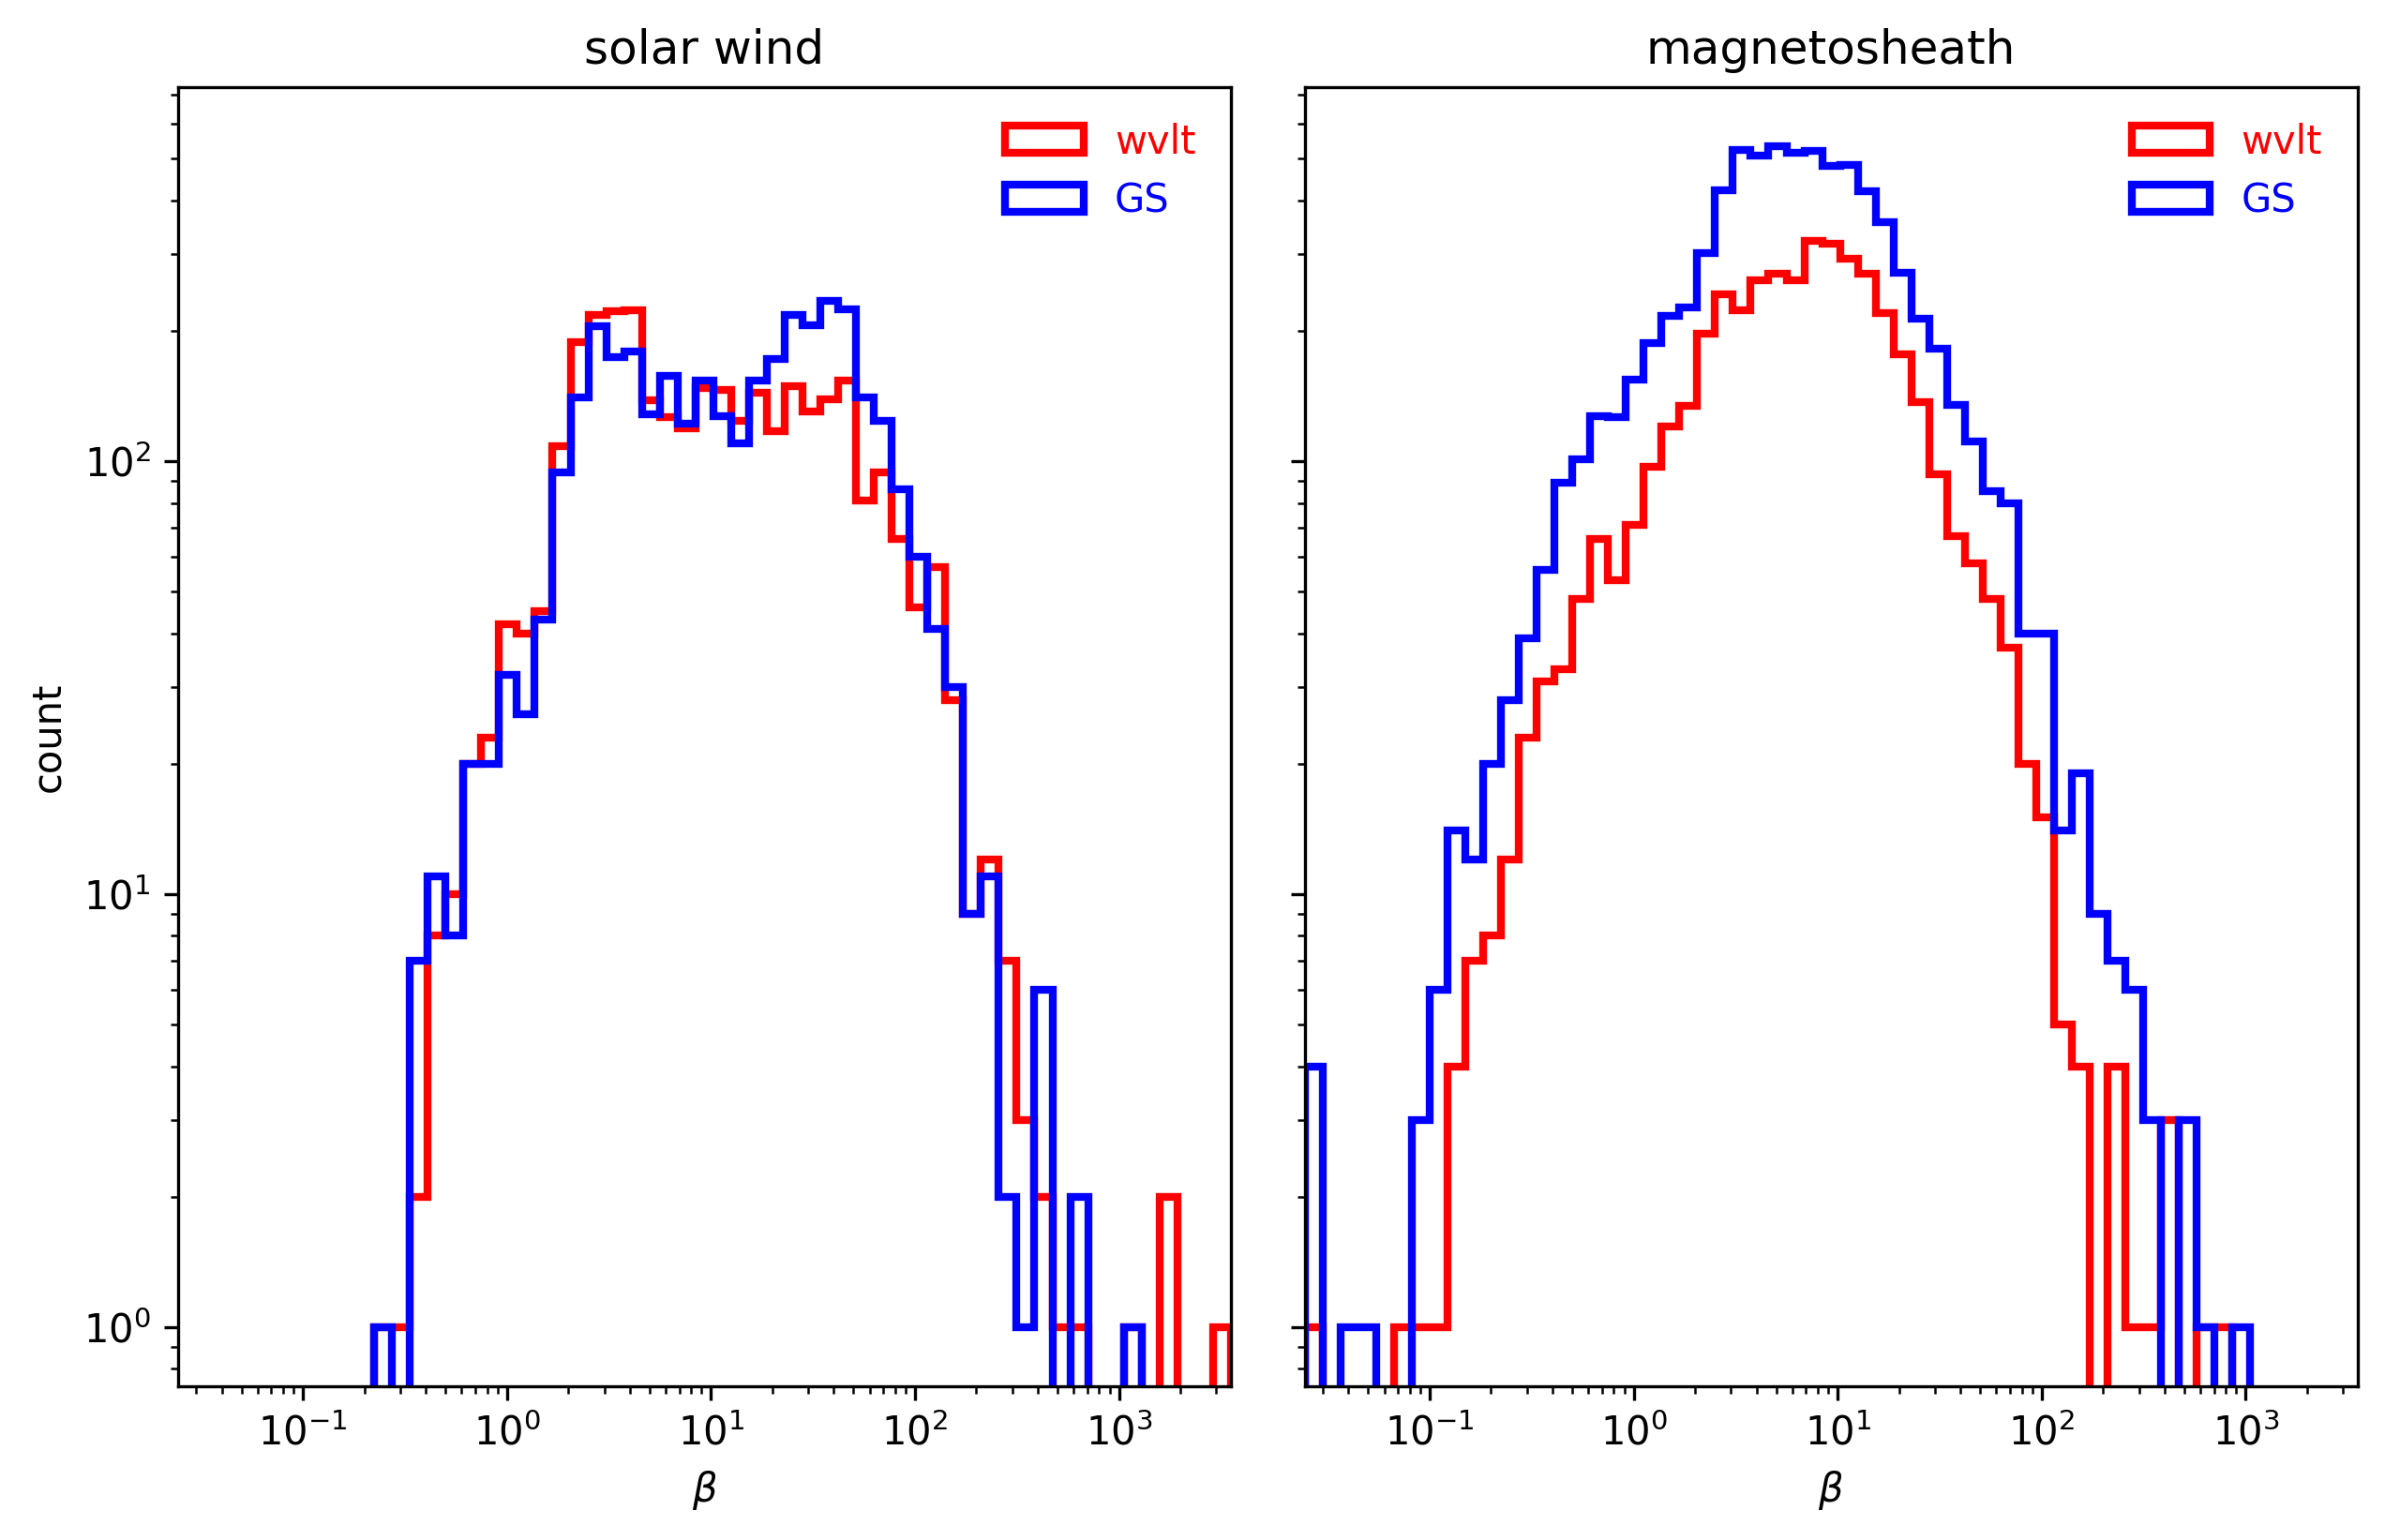
\includegraphics[width=\textwidth]{Figures/Histograms/histogram_logspace_beta.png}
    \caption[Histograms of beta for identified events]{Same as Figure \ref{fig:histogram-duration} but for plasma $\beta$ distributions of identified events.}
    \label{fig:histogram-beta}
\end{figure}

\begin{figure}
    \centering
    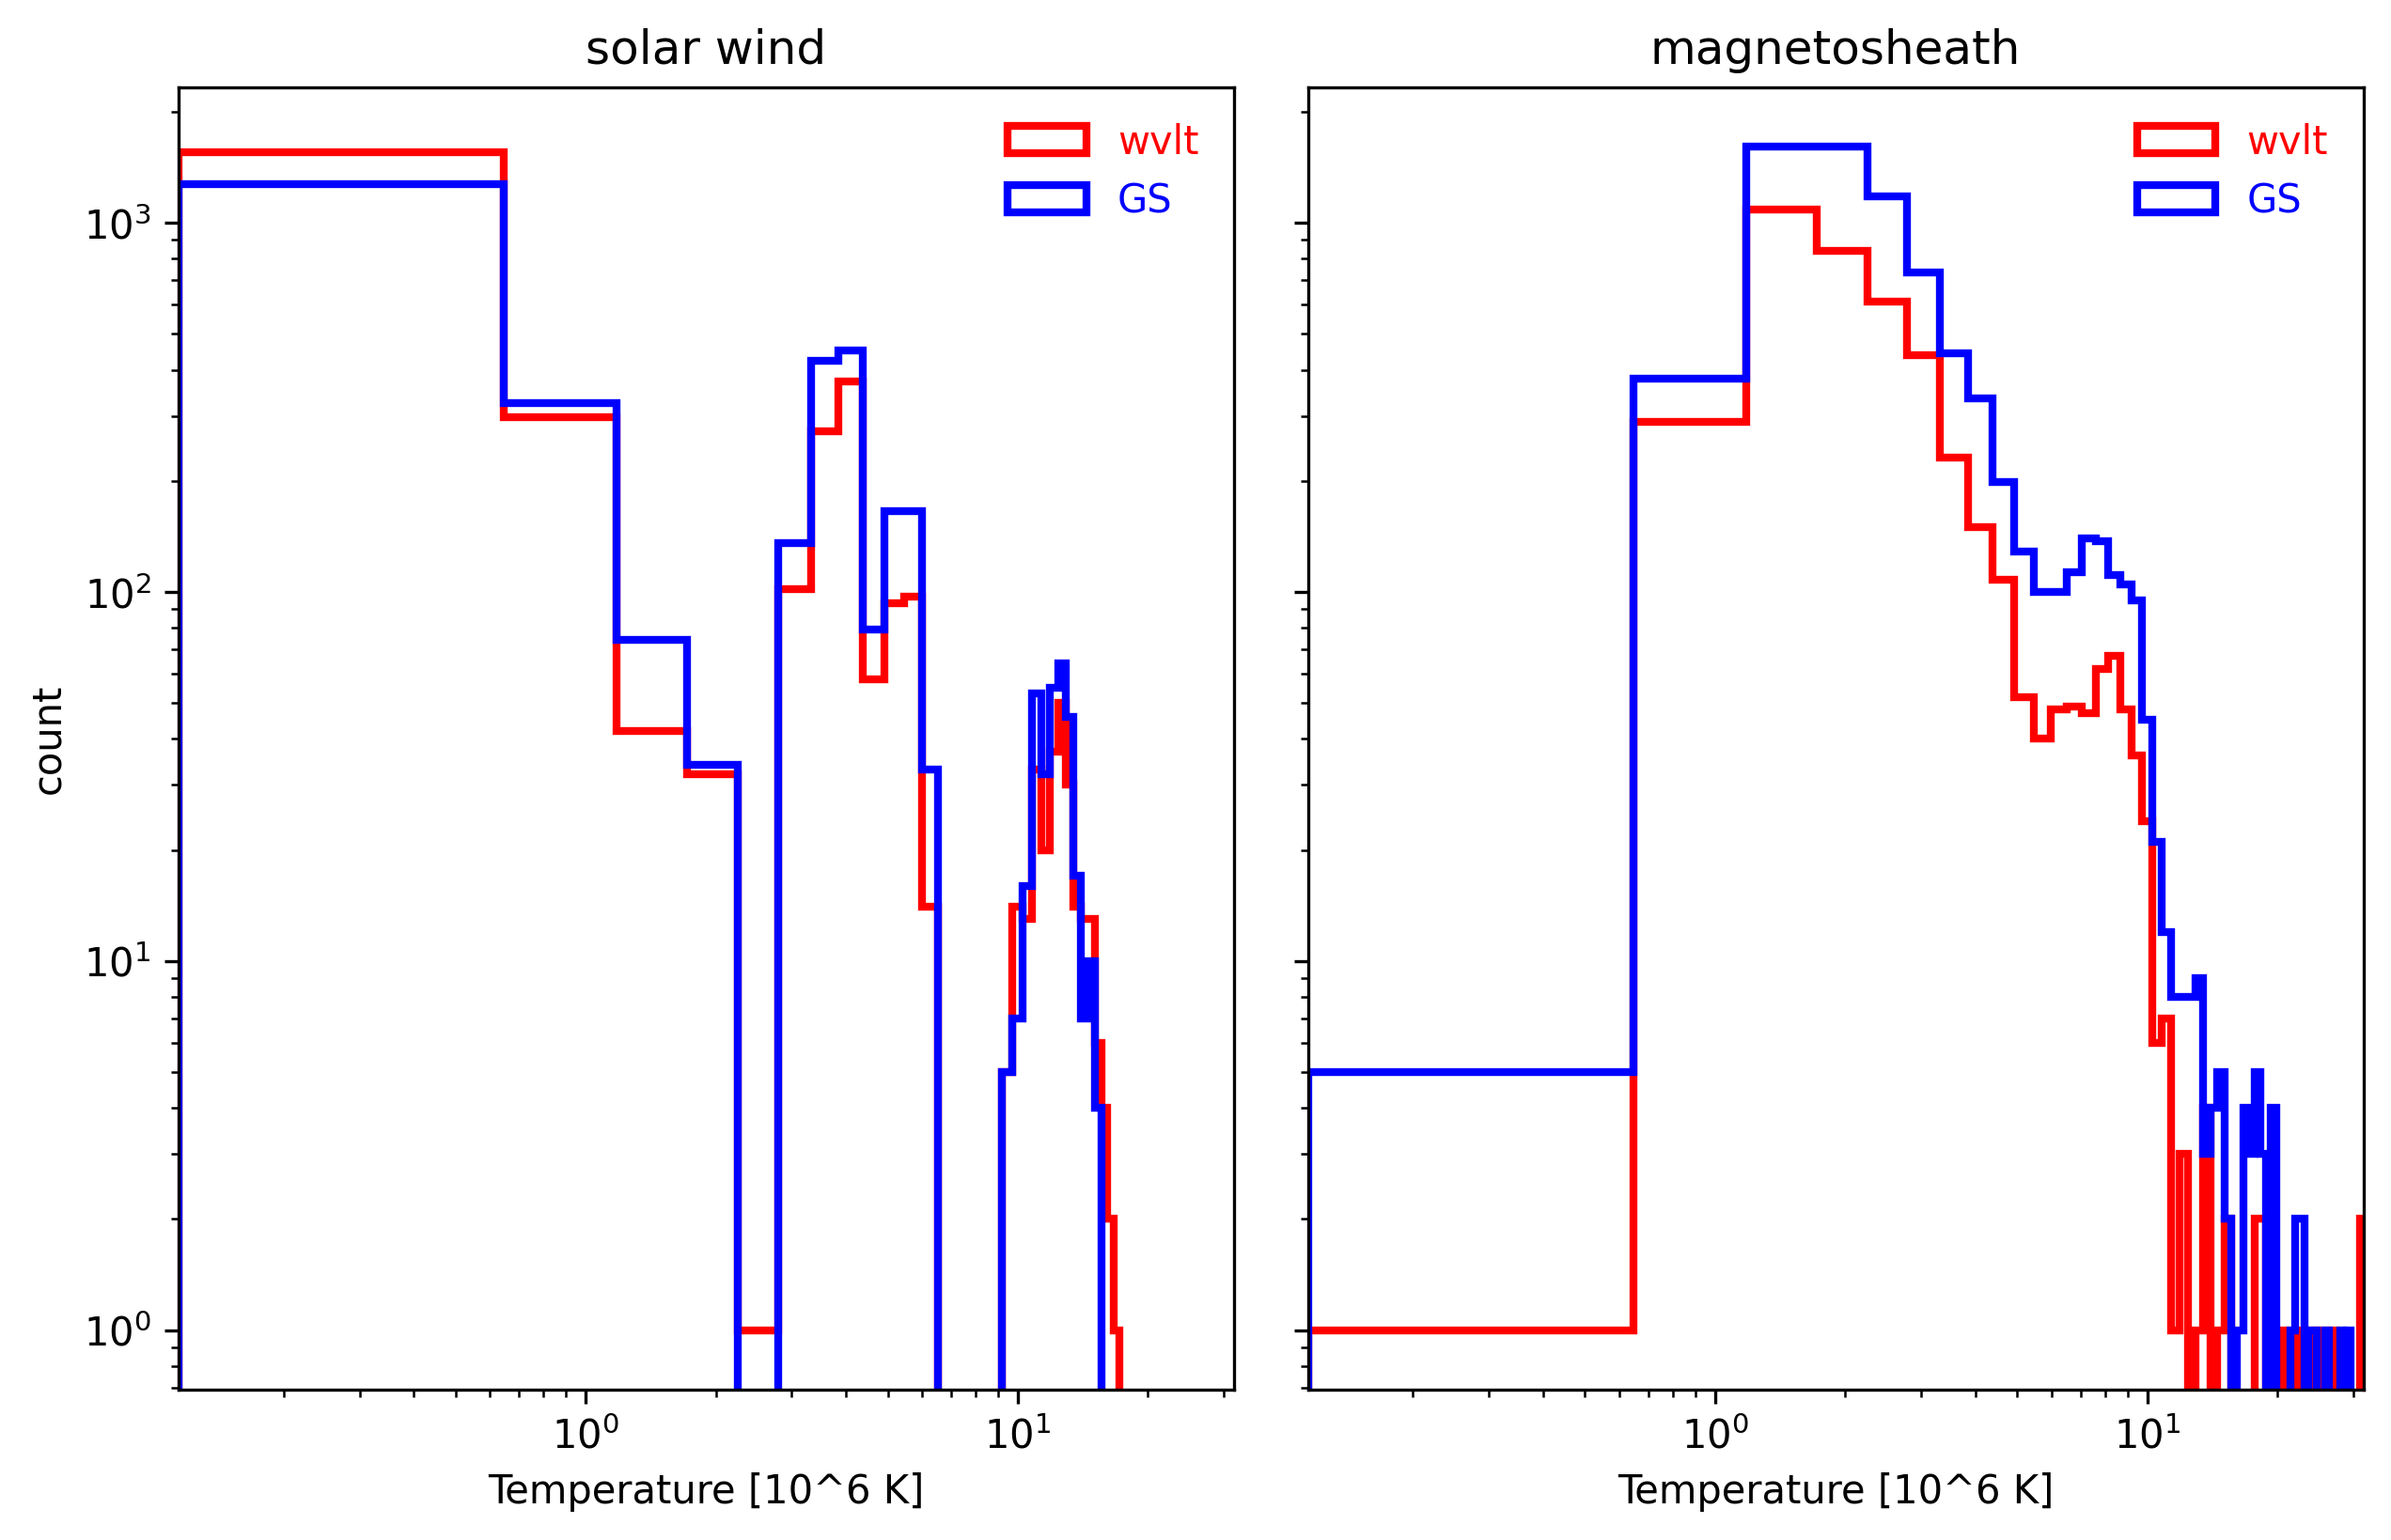
\includegraphics[width=\textwidth]{Figures/Histograms/histogram_temperature.png}
    \caption[Histograms of temperature for identified events]{Same as Figure \ref{fig:histogram-duration} but for temperature distributions of identified events.}
    \label{fig:histogram-temperature}
\end{figure}

\section{Summary}
In summary, we have carried out a comprehensive analysis of SFR structures in the regions immediately upstream and downstream of the Earth's bow shock. There were 11949 events identified in the magnetosheath across 1051 hours, with 7689 events being identified from the GS-based algorithm and 4260 from the wavelet analysis. For the solar wind, there were 6669 events identified across 676 hours, with 3476 being attributed to identification via the GS-based algorithm and 3193 via wavelet analysis. We utilized in situ observations of MMS-1, THM-A, THM-B, THM-C, and THM-E spacecraft. We extended the GS-based analysis to identify structures with significant remaining plasma flow aligned with the local magnetic field, and also performed wavelet analysis for 77 time periods in the solar wind and 130 time periods in the magnetosheath, corresponding to 676 hours and 1051 hours, respectively. The average magnetic field, velocity, duration, scale size, etc., of these structures were recorded for comparison. In addition to the general parameters, the GS-based method also yielded a unique set of additional parameters that allowed us to evaluate the distributions of the Wal\'en test slope, magnetic helicity density, magnetic flux, and the orientation of the $z$-axes of the structures.

We showed that the distributions of a wide variety of parameters generally follow power laws. The magnetic structures identified by the wavelet analysis were also characterized based on MHD quantities ($\sigma_m$, $\sigma_c$, $\sigma_r$). The different criteria assisted us to distinguish different types of events in terms of dynamic and quasi-static structures in the two regions. This work intended to examine the differences in the properties primarily obtained from the GS-based characterization of the identified SFR structures in the solar wind and magnetosheath. The additional findings of this study are summarized as follows.
\begin{enumerate}
    \item The magnitudes of the Wal\'en slope $|w|$ and cross helicity $\sigma_c$ parameters indicate the effect of the remaining plasma flow of the identified structures. Results from both regions indicate that about one-third of structures possess modest (e.g., $|w|>0.3$) remaining flow relative to the total number of structures identified.
    \item SFR structures are generally compressed downstream of the bow shock in the magnetosheath: the scale sizes are smaller while magnetic field strength increases in the magnetosheath. In addition, the magnetic helicity density per unit volume is about one order of magnitude larger than the corresponding value in the solar wind, implying an overall decrease in volume for the SFRs in the magnetosheath.
    \item A significant rotation in the polar angle of the $z$-axis in the magnetosheath is seen when compared to the angle in the solar wind, while the distributions of the azimuthal angle maintain two broad peaks separated by approximately 180 degrees. 
\end{enumerate}